\documentclass[12pt,a4paper]{article}
\usepackage{amsmath}
\usepackage{amsfonts}
\usepackage{amssymb}
\usepackage{graphicx}
\usepackage{secdot}
\usepackage{multirow}
\usepackage[left=2cm,right=2cm,top=2cm,bottom=2cm]{geometry}

\title{{Experiment - 10\\ \textbf{ Study of Boundary Layer over a rough flat plate}}}
\author{Arka Pramanick, AE21B007\\ Department of Aerospace Engineering\\ IIT Madras\\[3ex] Instructor:\\ \large Professor Dr. R. Sriram}

\date{26 April, 2023}


\begin{document}
\maketitle

\hline

\section{Aim :}
\begin{itemize}
    \item To Study Boundary Layer over a rough flat plate.
    \item To calculate Boundary Layer Thickness over the rough plate.
\end{itemize}


\section{Apparatus :}
Required apparatus for performing this experiment are:
\begin{itemize}
    \item Manometer
    \item C15-10 Armfield tunnel
    \item Pitot-static Probe
    \item Rectangular rough flat Plate
\end{itemize}



\newpage
\section{Theory :}

\subsection{Boundary Layer :} The phenomenon of boundary layer is a thin layer near to a surface where viscous effects are significant.Fluid flowing over a solid surface occurs no slip condition when the fluid particle sticks to stationary surface boundary;which results in  velocity of fluid near to the boundary equal to the boundary.The velocity of fluid increases from zero (on the stationary 
boundary) to the free stream velocity($V_{\infty}$) of the fluid in the direction normal to the boundary. In rough flat plates creates negative pressure provides some angle to the particular roughness.Thickness of boundary layer increases on increasing inclination of the flat plate due to generation of vortex formation and consequent turbulence.\\
For a body over which the fluid flows, close to the body is the boundary layer where shear stresses exert an increasingly larger effect on the fluid as one moves from free stream towards the solid boundary.Outside the boundary layer where the effect of the shear stresses on the flow is very small compared to values inside the boundary layer (since the velocity gradient $ \frac{\delta u}{\delta y} $ is negligible) .
\subsection{Boundary Layer Thickness :} Boundary Layer thickness is the thickness where velocity approaches to free stream Velocity.The velocity in boundary layer  increases in an asymptotic manner.




\begin{figure}[!ht]
	\begin{center}
		\framebox{
			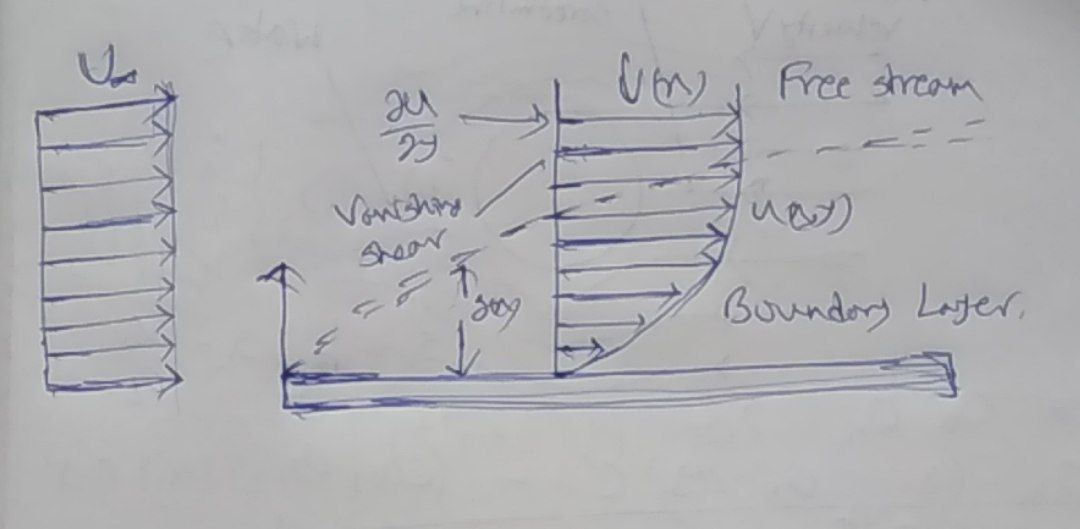
\includegraphics[scale=0.3]{photo_6221772200483075255_y.jpg}
		}
	\end{center}
	\caption{Formation of Boundary Layer with generation of Velocity gradient}
\end{figure}





\section{Procedure :}
\begin{enumerate}
    \item In wind tunnel test section is set.
    \item Rectangular Surface is fixed inside wind tunnel.
    \item Pitot-static probe is connected to manometer.
    \item Fan speed is fixed.
    \item Required readings are taken to calculate Boundary Layer Thickness.
\end{enumerate}






\section{Observation :}


\subsection{Table for Y distance and Velocity :}
\begin{table}[ht]
\centering
\vspace{2mm}
\begin{tabular}{|c|c|c|} 
 \hline
Y Distance (in mm) & Stagnation Pressure($P_{stag})(in Pa)$ &  Velocity (m/s) \\ 
 \hline
 0 & -65 & 11.30 \\
 \hline
0.5 & -65 & 11.30 \\ 
 \hline
 1 & -63 & 11.44 \\
 \hline
1.5 & -62 & 11.52  \\
 \hline
2.0 & -61 & 11.59 \\
 \hline
2.5 & -60 & 11.66 \\ 
 \hline
3.0 & -58 & 11.80 \\ 
 \hline
 3.2 & -52 & 12.20 \\
 \hline
3.4 & -44 & 12.73  \\
 \hline
3.6 & -40 & 12.98 \\
 \hline
3.7 & -37 & 13.17 \\ 
 \hline 
3.8 & -35 & 13.29 \\
 \hline
3.9 & -33 & 13.41 \\ 
 \hline
4.0 & -31 & 13.54 \\
 \hline
4.1 & -31 & 13.54 \\ 
 \hline
4.2 & -29 & 13.65 \\
 \hline
4.3 & -27 & 13.77  \\
 \hline
4.4 & -27 & 13.77 \\
 \hline
4.5 & -26 & 13.83 \\ 
 \hline 
4.6 & -27 & 13.77 \\ 
 \hline
4.7 & -25 & 13.89 \\
 \hline
4.8 & -25 & 13.89  \\
 \hline
4.9 & -25 & 13.89 \\
 \hline
5.0 & -25 & 13.89 \\ 
 \hline 
 \end{tabular}
\end{table}

 \subsection{Data for Boundary Layer Thickness for different Velocities for measurements at 80 mm and 120 mm from leading edge.}

 \underline{For measurements at 80 mm from Leading edge} :
\begin{table}[ht]
\centering
\begin{tabular}{|c|c|c|}
 \hline
Velocity(m/s) & Reynolds No.(Re) & Boundary Layer Thickness(mm)   \\
\hline
8 & 40736 & 1.2 \\
\hline
10 & 51879.3 & 1.1 \\
 \hline
12 & 65261 & 1.3 \\
\hline
14 & 75801 & 2.5 \\
\hline
16 & 86629.83 & 1.73 \\
\hline
18 & 124410 & 4.3 \\
\hline
\end{tabular}
\end{table}

 \underline{For measurements at 120 mm from Leading edge} :
\begin{table}[ht]
\centering
\begin{tabular}{|c|c|c|}
 \hline
Velocity(m/s) & Reynolds No.(Re) & Boundary Layer Thickness(mm)   \\
\hline
8 & 58006 & 1.5 \\
\hline
10 & 73231.66 & 1.5 \\
 \hline
12 & 97458.56 & 2.1 \\
\hline
14 & 113702 & 2.25 \\
\hline
16 & 129729.73 & 3.7 \\
\hline
18 & 162431 & 4.2 \\
\hline
\end{tabular}
\caption{Caption}
\end{table}





\subsection{Plot of Displacement thicknesses vs Velocity : } 



\begin{figure}[!ht]
	\begin{center}
		\framebox{
			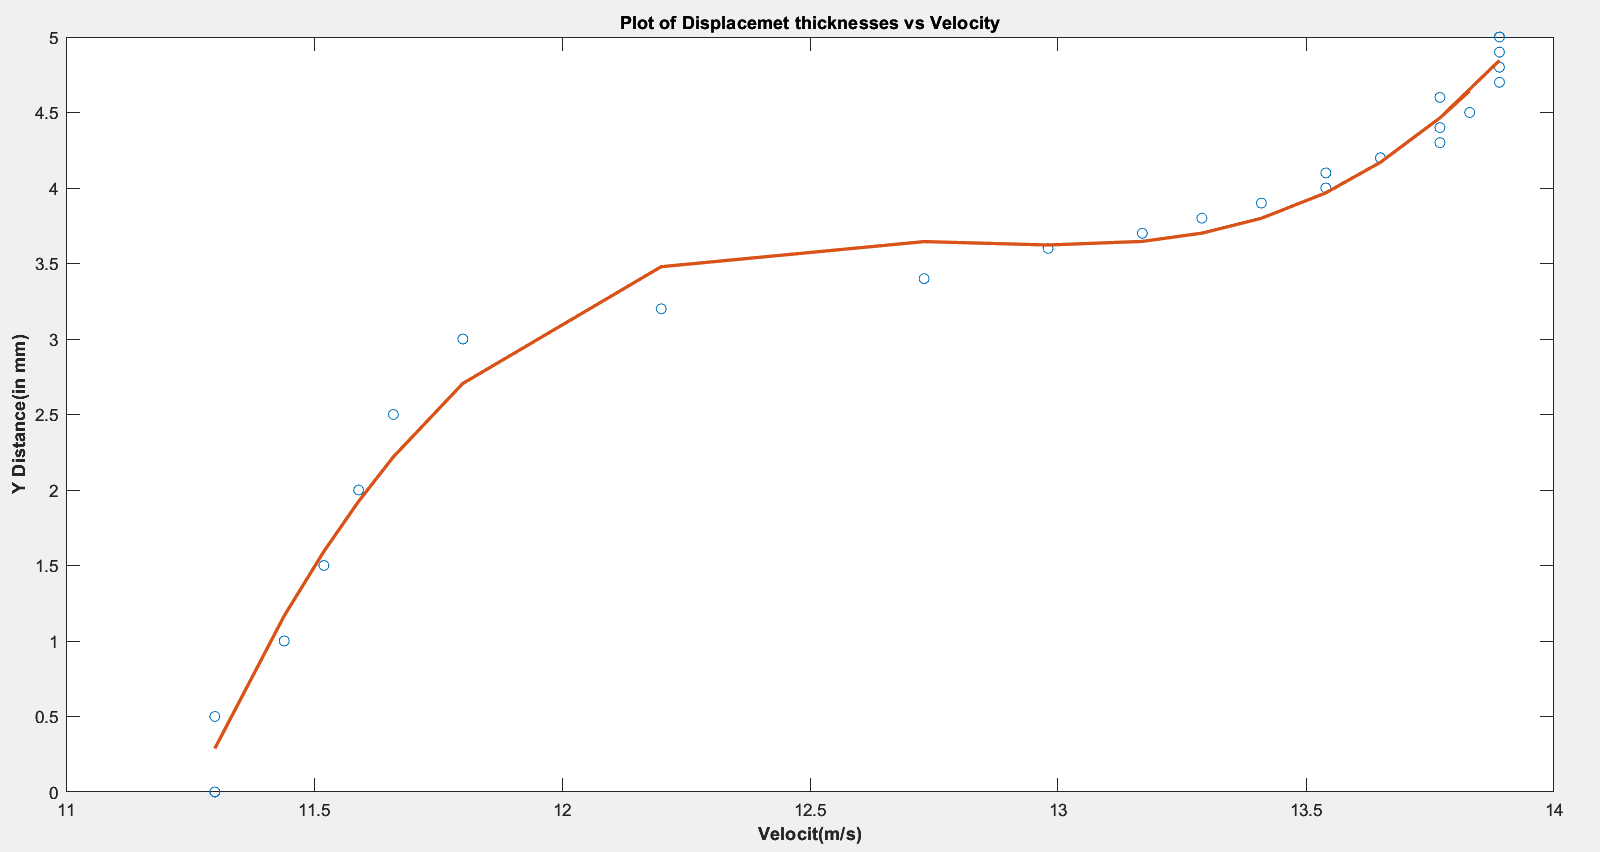
\includegraphics[scale=0.42]{displacement thickness.png}
		}
	\end{center}
	\caption{Variation ofY Distance with Velocities}
\end{figure}

\subsection{Plot of Boundary Layer Thickness vs Reynolds No. at two different positions from Leading Edge}
\begin{figure}[!ht]
	\begin{center}
		\framebox{
			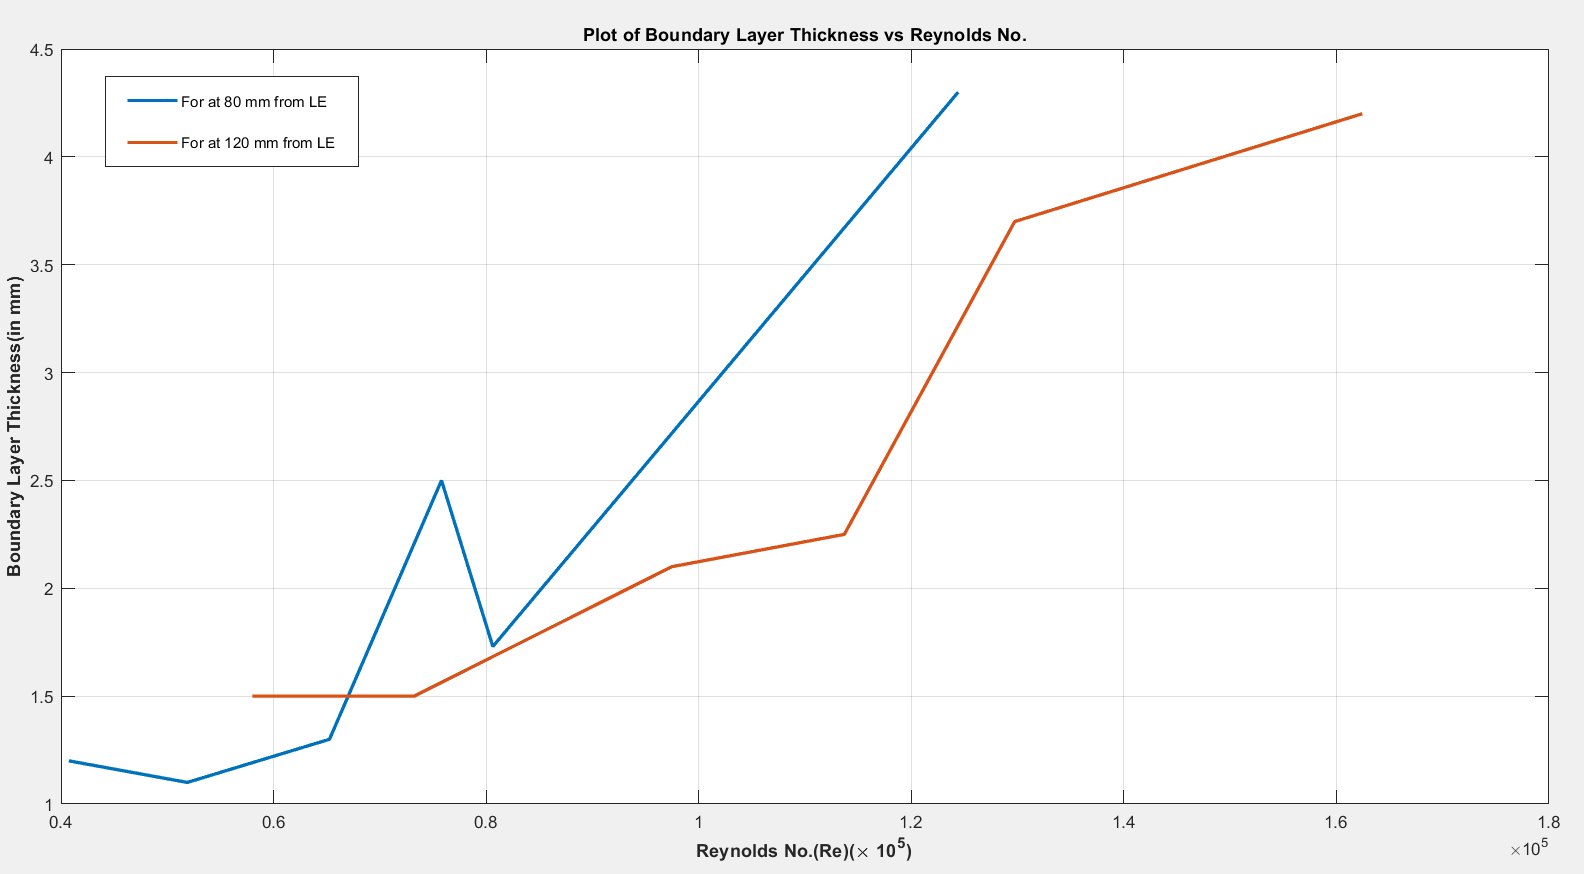
\includegraphics[scale=0.65]{BLT VS RE.png}
		}
	\end{center}
	\caption{Variation of Boundary Layer Thickness with Reynolds No. at two different positions from Leading Edge}
\end{figure}


\section{Calculations :}
Density of air($\rho$) = 1.225 $\frac{Kg}{m^3}$ \\
Density of Water($\rho_w$) = 1000 $\frac{Kg}{m^3}$ \\
Static Pressure ($P_{stat}$) = 14.6 mm of Water = 143.226 Pa
Measurement at a position at a distance(L) = 80 mm from Leading Edge.
$V_{\infty}$ = 16 m/s
Viscosity ($\mu$) = $1.81 \times 10^{-5}$

\subsection{Calculation of Velocity :}
At 0 mm ,
Stagnation pressure ($P_{stag}$) = -65 Pa \\

$$ P_{stag} = P_{stat} + \Delta P $$ 
$\Delta P = Dynamic Pressure = \frac{\rho V^2}{2}$ \\
$$ V = \sqrt{\frac{2(P_{stag}-P_{stat})}{\rho}} $$
$$ V = \sqrt{\frac{2(-65+143.226)}{1.225}} $$
$$ V = 11.30 m/s $$

\subsection{Calculation of Displacement Thickness:}

Displacement thickness = ($\delta^{\ast}$) = \[ \int_{0}^{\infty} (1-\frac{V}{V_{\infty}}) \,dx \]
$$ \delta^{\ast} \approx \sum_{n=0}^{\infty} (1-\frac{V}{V_{\infty}})t $$
$$ \delta^{\ast} = 1.73 mm $$ 
Therefore displacement thickness ($\delta^{\ast}$) = 1.73 mm

\subsection{Calculation of Momentum Thickness:}
$$ \theta ^{\ast} = \int_{0}^{\infty} (1-\frac{V}{V_{\infty}})(\frac{V}{V_{\infty}}) \,dx $$
$$ \theta^{\ast} \approx \sum_{n=0}^{\infty} (1-\frac{V}{V_{\infty}})(\frac{V}{V_{\infty}})t $$
$$ \theta^{\ast} =1.46 $$
Momentum thickness($\theta^{\ast}$) = 1.46 

\subsection{Calculation of Reynolds No.(Re) :}
$$ Reynolds No.(Re) = \frac{\rho V_{\infty} L}{\mu} $$
$$ Re = \frac{1.225\times16\times.08}{1.81 \times 10^{-5}} $$
$$ Reynolds no. = 86629.83 $$


\section{Sources of Error:}
\begin{itemize}
    \item Error due to instrumental defect.
    \item Error may occur in taking readings before flow becomes steady.
    \item Error due to environmental effect like temperature,pressure change.
    \item Error in measurement due to presence of zero error in parameters.
    \item Dimensional error may occurs .
    \item Parallax error may occur.
\end{itemize}



\section{Conclusion :}
\begin{itemize}
    \item Velocity of flowing fluid increases as we move away from boundary/surface of the object.
    \item Velocity of fluid near the boundary is same as that of boundary.
    \item Closer to the Leading edge slope of BLT(Boundary Layer Thickness) and Reynolds No. become more stiffer.
    \item Boundary Layer Thickness increases on increasing Reynolds No.
\end{itemize}


\end{document}